\documentclass[11pt]{article}
% Target: Nature Machine Intelligence, Article.
% Main text (intro + Results + Discussion) <= 3,500 words; abstract <= 150 words;
% <= 6 display items. Methods, references and legends sit outside the limit.

\usepackage[utf8]{inputenc}
\usepackage[T1]{fontenc}

\usepackage[margin=1in]{geometry}
\usepackage{amsmath,amssymb}
\usepackage{graphicx}
\usepackage{booktabs}
\usepackage{xcolor}
\usepackage{setspace}
\usepackage{caption}

\usepackage[super,sort&compress,comma]{natbib}
\usepackage{lineno}
\usepackage[hidelinks]{hyperref}



\DeclareCaptionLabelSeparator{bar}{ | }
\captionsetup{font=small,labelfont=bf,labelsep=bar,justification=raggedright,singlelinecheck=false}
\renewcommand{\figurename}{Fig.}
\renewcommand{\bibnumfmt}[1]{#1.}
\graphicspath{{figures/}}
\onehalfspacing
\setlength{\emergencystretch}{2em}
\linenumbers

\title{\textbf{Stateless weights, stateful store:\\ memory as a block inside the transformer}}
\author{Adhavan K,\textsuperscript{1} Prem Vaishnav P\textsuperscript{1} and Vinila Jinny S\textsuperscript{1,*}\\[4pt]
\small \textsuperscript{1}School of Computer Science and Engineering, Vellore Institute of Technology, Vellore, India\\
\small \textsuperscript{*}Corresponding author: Dr Vinila Jinny S, vinilajinny.s@vit.ac.in\\
\small ORCID 0000-0003-2756-6736}
\date{}

\begin{document}
\maketitle

% abstract  -  part of main.tex (see journal/README.md)
\noindent Language models forget everything between conversations, so long-term memory is
usually bolted on outside the network. We put it inside instead. A memory block in the
transformer reads from and writes to a persistent store addressed by each word's identity,
so retrieval is an exact match. State then lives in the store: one frozen model is a
different agent with each store it loads, and swapping stores swaps the memory without
touching a weight. Facts stated once in text are recalled out of context at 99--100\% for
up to 64 facts, while controls sit at chance. A read touches one slot per query, and recall
survives a million tokens. Nothing is lost in the middle, although facts written late into
a full store are. The store revises facts, stays bounded, and supports reasoning across up to
five stored facts.
\par\bigskip

% introduction  -  part of main.tex (see journal/README.md)
A transformer carries no state from one call to the next. Everything it knows about a
conversation has to be supplied again in its prompt, the window of text it reads at once
\cite{vaswani2017attention}. Systems that give language models long-term memory therefore
treat memory as a layer of engineering wrapped around a frozen network: text is embedded,
stored in an external database, retrieved by similarity and pasted back into the context
window\cite{lewis2020rag,packer2023memgpt,park2023generative}. That works, but it ties
recall to the context budget, leaves the model itself stateless, and hands memory to the
harness instead of the model. Memory-augmented architectures move memory inside the network
instead---as recurrent or compressed
state\cite{dai2019transformerxl,rae2020compressive,bulatov2022rmt}, as a memory bank read
and written by attention\cite{graves2014ntm,graves2016dnc,weston2015memnet,sukhbaatar2015e2e,wu2022memformer},
or as a cache of past attention keys searched by nearest neighbour\cite{wu2022memorizing}.
That memory is bound to one sequence, is addressed by contextual representations that drift
during training, and is not a portable artefact of the model.

We ask whether memory can be part of the model. We add one memory block inside the stack
(Fig.~\ref{fig:arch}a). Every layer reads from, and writes its own state into, a single
persistent store shared across layers. The store's address is the raw embedding of each
token (a word or word fragment) at layer~0, before any processing and without position
information, so retrieval is an exact token match. Text is processed in fixed segments,
and the model keeps no key--value cache (the attention state a
transformer would otherwise carry forward) between them, so the store is the only channel
from one segment to the next.

The design puts the weights and the store in separate roles. The weights are stateless and
the store is the state. A frozen model carries nothing of a conversation; all of it lives in
a detachable file. We show this literally: swapping the store swaps the memory without
changing a weight (Fig.~\ref{fig:arch}b). We also show where the property stops. A store can
be read only by the model that wrote it.

Across 113 controlled experiments, we find that this block
(i)~recalls facts stated once in natural-language text and queried entirely out of context,
and keeps them across a process restart; (ii)~holds facts far beyond the attention window,
read by touching a single slot, with recall flat to a million tokens and no lost-in-the-middle
effect (the weaker retrieval of facts placed mid-context\cite{liu2024lost}); (iii)~can be
revised, bounded and reasoned over, which turns a lookup table into a memory; and
(iv)~maps onto the shared key--value constructions now used to compress attention
caches\cite{deepseekv41flash2026}. We also locate where it fails. A single store saturates
near 128 distinct facts, and a fact written late into a saturated store is lost. Both limits
come from addressing and from the write policy. Position is not the problem.

% results  -  part of main.tex (see journal/README.md)
\section*{Results}

\subsection*{A memory block addressed by the token itself}

The block has three parts (Fig.~\ref{fig:arch}a, Methods and Supplementary Note~1). A \emph{key} is the
token's layer-0 embedding without position, and the read head's query projection is
initialised to the identity and frozen, so a token matches itself exactly. A \emph{read} scores the stored
keys by cosine similarity, sharpens the scores by an annealed softmax in the manner of a modern Hopfield network\cite{hopfield1982,ramsauer2021hopfield} (an associative memory that returns the stored pattern closest to a cue), and injects the blended values into the residual stream (the running representation that every layer reads and updates) through a gate initialised at zero\cite{bachlechner2021rezero}.
At initialisation the block is therefore an exact no-op, and the store-disabled model is a
true control. A \emph{write} stores one slot per token, with the value shifted by one
position so that the slot keyed on a token returns what followed it.

Where reads and writes happen matters. Writing the mean of all layers' states into one slot
per token gives 80.8\% recall on a 32-fact task. Letting every layer write its own
post-block state as its own slot in the one shared store lifts this to 95.5\% and 98.9\% over two seeds (Table~\ref{tab:core}; Supplementary Note~2 and Supplementary Table~1). A control with the same
number of slots, but keyed by each layer's evolving residual, stays at
0.2\%. The gain comes from per-depth values that stay exactly addressable. Extra capacity
on its own does not do it. The exact address is load-bearing. Every attempt to enrich the
key---moving it deeper, adding position, mixing in a neighbouring token, or projecting it to
fewer dimensions---collapsed matching to chance (Supplementary Note~2).

\subsection*{Recall of facts stated once, out of context}

We test memory with a task in which no answer can come from the prompt (Supplementary Note~3). The first segment
states $n$ key--value facts inside PG-19 prose (a corpus of books)\cite{rae2020compressive}; intermediate
segments are unrelated prose; the final segment holds only a query marker and one key. Two
matched controls run every time: the store disabled, and a scrambled store in which each
example reads a neighbour's store.

With single-token sub-word keys\cite{sennrich2016bpe}, recall is 100\% at 8, 16 and 32
facts and 99.1\% at 64, with the scrambled control at $0.16\%$ (Table~\ref{tab:core}; Supplementary Table~2).
Memory survives the process: a store written, then reloaded in a fresh interpreter, answers
at 100\%, and a mismatched store file at $0.0\%$. Two obstacles had to be removed on
the way. Character-level keys impose a \emph{multi-token-key tax}: the only token at the
retrieval point is a shared delimiter, so recall falls from
90\% to 55\% between 4 and 13 facts; a single-token key removes it. The
familiar fact-count cliff---recall collapsing beyond a threshold even though the top-scoring
slot is correct---is a training-dynamics deadlock rather than a capacity limit. Multi-layer
placement clears it from a cold start after a delayed phase transition (99.7\% at 16
facts, 98.0\% at 32), and a warm-start curriculum reaches the same endpoint in about
half the steps.

\subsection*{The weights are stateless; the store is the state}

Splitting weights from store predicts that a store can be moved between conversations
without touching the model. We hold one trained model fixed and build two stores from
disjoint fact sets (Fig.~\ref{fig:arch}b and Supplementary Note~4). Recall
is diagonal: 100\% and 96.9\% when the store that holds the queried facts is
loaded, and $0.0\%$ when the other store is, with a scrambled store at chance (one of 32 queries, $3.1\%$; Table~\ref{tab:core} and Supplementary Table~3). Swapping the store swaps the memory.

The same experiment marks the boundary. Two independently seeded models each read their own
store at 98.8\% and 100\%, but each other's at $0.0\%$, in both directions,
although the facts are physically present and the stores are shape-compatible. A store's
keys are its writer's token embeddings, so a store is a memory only for the model that wrote
it, and the persistence path refuses a foreign store by its model fingerprint. One frozen
model can therefore serve many users by loading their stores. Carrying memory across model
versions requires re-encoding, which is cheap: the stored keys decode exactly to their
tokens, so the key sequence is itself the transcript of what was written (Methods).

\subsection*{Memory far beyond the attention window}

Because the store sits outside attention, it can span many attention windows. A fixed ring
buffer eventually overwrites old facts, which is a limit of eviction policy and not of
capacity. We
instead grow the store by appending, like a key--value cache, and read it with a top-1 lookup, which uses only the best-matching slot (Supplementary Note~5). Recall then stays at 100\% from 1.9k to 998k tokens between fact and query (Fig.~\ref{fig:long}a and Supplementary Table~4), about 7,800 times the 128-token window, on both a
two-layer and a six-layer model. A dense read over all slots decays as distractors
accumulate, from 85\% to 60\% by 25k tokens and to $0\%$ by 128k, so sparse reading is a
requirement, not a compromise. A scrambled store sits at $0.0\%$ at 128k and 384k tokens.
Reaching a million tokens needed an evaluation-time change only: building the store in place
rather than rewriting it every segment (Methods). The read is $O(1)$ per query, so build time
sets the reach. One caveat runs the other way. Keys drawn from
the rarest words, whose embeddings are least trained, recall at 50--75\% even at a million
tokens. That is an effect of embedding quality, not of store size.

The store also behaves as a shared key--value memory in the sense used to compress attention caches\cite{shazeer2019mqa,ainslie2023gqa,deepseekv2mla2024,deepseekv41flash2026} (Supplementary Note~6). An index of
each slot's key token lets a query score about 2 of 8,001 slots at the recall of a dense scan
(81.9\% versus 82.5\%; Supplementary Table~5). Building that candidate pool once and reusing it at every read layer
gives recall identical to rebuilding it per layer. The stored codes survive quantization (storing numbers at reduced precision) to 4 bits per element with no loss (Fig.~\ref{fig:long}b), eight times smaller than the
32-bit store. Keys are the
bit-limiting half: they fail at 3 bits, while values hold to 3. Both figures are measured
properties of the read. Turning them into speed and memory savings needs specialised low-level routines for hashed lookup and 4-bit integers.

\subsection*{No lost-in-the-middle, but a write-order limit}

Attention models retrieve facts placed in the middle of a long context worse than those at
its ends\cite{liu2024lost}. We tested this with a passkey design\cite{mohtashami2023landmark}, in which a fact is planted at a chosen depth in long filler text and queried at the end, varying that depth (Supplementary Note~5). The store shows no mid-context dip:
recall is monotonic in depth (Fig.~\ref{fig:passkey}a). In its place there is a \emph{write-order}
decay that grows with saturation. A fact written first stays at 100\%, but a fact
written last falls from 81\% to 50\% to 6\% as the store fills from 4k to 16k to 65k slots,
with a scrambled store at $0\%$ throughout. The store privileges what it saw first, the
opposite of a recency bias.

Two ablations locate the cause (Fig.~\ref{fig:passkey}b). Ring overwriting is not the
explanation: an append-only store gives an identical curve. The write policy is part of it. The block stores a
segment only when it is novel enough relative to the store (Methods), and a late fact whose
key token recurs in the intervening prose reads as familiar. Keying facts on unique tokens,
which always read as novel, lifts the late tail fourfold, from 6\% to 25\%, though it lowers
the early end from 100\% to 75\% because rarely seen tokens have weaker embeddings. On a
weaker six-layer model the decay is nearly binary: only the first-written fact survives,
and unique keys do not help (Fig.~\ref{fig:passkey}c). The limit is part fixable write
policy, part saturation, and nothing to do with position.

\subsection*{From a lookup table to a memory}

A store that can only be appended to and read is a lookup table. A memory must also revise a
fact when it is restated, stay bounded as text accumulates, and support computation over its
contents. We added each by changing only the read and write heads (Fig.~\ref{fig:memory}; Supplementary Note~7 and Supplementary Table~6).

\emph{Revision.} An append-only store keeps both the old and new value of a restated fact and
cannot tell which is current. A small bias towards the most recently written match, read from
a global write counter, lifts newest-value recall from 88.9\% to 96.7\%, while facts that were never updated stay at 97.5\% (Fig.~\ref{fig:memory}a). The
position-free key carries no recency of its own; recency has to come from write order.

\emph{Boundedness.} Gated write operations keyed on the token---\textsc{new},
\textsc{update-in-place} or \textsc{skip}---keep one slot per distinct fact. Recall is
95.9\% at about 200 occupied slots against 94.1\% at 508 when every occurrence
is appended, and updates land at 96.2\% against 7.8\%
(Fig.~\ref{fig:memory}b). A single shared store with these operations matches separate
per-layer stores (96.2\% recall, 96.6\% update).

\emph{Composition.} Given $A\!\to\!B$ and $B\!\to\!C$ stored beyond the window, answering $A$
with $C$ needs two retrievals chained through the store. Feeding a retrieved representation
back as the next query failed in all seven variants we tried, at chance: a stored value does
not lie on the manifold of keys, so the next exact match never fires. Composition works
as a working-memory operation. The model emits each intermediate as a token and
queries again, a chain of thought\cite{wei2022cot} (writing out intermediate steps) whose steps are store reads. Joint recall
is 96.9\% at two hops and 95.2\% at three over 64 facts, and 91.6\% at
four and 89.7\% at five over 32 facts, close to 0.98 per hop (Fig.~\ref{fig:memory}c). Feeding the model its own emitted intermediates, in place of the true
ones, changes nothing. Breaking one link of the chain drops joint recall to $0.0\%$ while
the preceding hops still succeed, so the model is composing rather than taking a shortcut.

\emph{Meaning.} The exact match is not semantic. A synonym of a stored key retrieves at
chance (about 4\%), and softening the read narrows what matches further. Meaning
can come from reasoning instead. When the first hop maps a synonym to its canonical form from
the weights and the second hop reads the store, synonym-queried facts are recalled at
90.8\%; replacing the synonym map with a random, unlearnable one drops the first hop
to 2\%. The store is an exact index, and meaning is supplied above it.



% discussion  -  part of main.tex (see journal/README.md)
\section*{Discussion}

Memory can sit inside the model instead of around it. The weights compute and the store
remembers, and because the store is addressed by the token itself, retrieval is exact and
cheap: a read touches one slot, even for facts a million tokens back. The store is also
just a file, so it can be swapped, persisted or deleted. Revision, boundedness, composition and
meaning all come from gating and reasoning layered above it. The arrangement
resembles complementary-learning-systems accounts of the brain, in which a fast, index-like
hippocampal store sits beside slowly learning cortex\cite{teyler1986indexing,mcclelland1995cls,kumaran2016cls}.
The analogy holds in one further respect: an offline replay phase moves stored episodes
into the weights, using the store's own key sequence as the transcript (Supplementary Note~8).

Compared with earlier memory-augmented transformers, this trades space for exactness.
Recurrent and compressed memories\cite{bulatov2022rmt,rae2020compressive,wu2022memformer} hold
a fixed-size summary in constant space, so a fact mentioned once can be blurred or
overwritten. Ours does the opposite: it grows, keeps exact content, stays cheap to read,
and outlives the sequence and the process that wrote it. Every experiment, including the designs we
tried and discarded, is recorded with its hypothesis and result in Supplementary Data~1.

The limits are worth stating plainly alongside the results (Supplementary Note~9). Scale is the first
of them: every model here has 7.8--12.1 million parameters, and the larger-scale runs are
pending. Then capacity. A single shared store binding 128 distinct facts saturates
near 45\%, and neither more attention heads, a curriculum nor a 3.4-fold wider model closes
the gap (44--48\%). We believe this is an addressing limit of the kind that positional
encodings resolve in a key--value cache. A positional or ordinal tag applied symmetrically
to query and stored key would separate colliding facts without disturbing the exact match.
The recency read is a first instance of such a tag. Part of the write-order limit is a
fixed novelty gate, which points towards learning what to store. Our efficiency results
stop at measurement; nothing has been realised in specialised hashed and 4-bit kernels.
Most of what we report is controlled recall over natural prose, and the standard long-context
benchmarks\cite{kuratov2024babilong,hsieh2024ruler} are part of the pending work.

A model whose memory is a file changes what you can do with it. Memory becomes something
you can load per user, inspect by decoding its keys, and delete outright; deleting a store
removes whatever has not been consolidated into the weights. The split we use here,
stateless weights and a stateful store, is a practical way to build models that remember.

% methods  -  part of main.tex (see journal/README.md)
\section*{Methods}

\paragraph{Model.} We use small decoder-only transformers with byte-pair-encoded
vocabularies of 8,192 tokens trained on PG-19\cite{rae2020compressive}, in four shapes, each
with a single attention head: $d_\text{model}=256$ with 6 layers (the default; 7.8M parameters),
512 with 2 (12.1M), 384 with 3 (9.7M) and 192 with 12 (7.9M). Text is processed in segments of 128
tokens. The forward pass is stateless per segment and keeps no key--value cache across
segments, so the store is the only cross-segment channel.

\paragraph{Memory block.} For each token the key is its layer-0 embedding without position
information. Each read head projects the layer's hidden state to a query; the projection is
initialised to the identity and frozen, so a token's query equals its key. A read computes
cosine scores between the query and every stored key (after subtracting a running key mean),
sharpens them with a softmax at inverse temperature $\beta$ (32 at inference), and returns the
score-weighted sum of stored values, projected back to the model width and added to the
residual stream through a scalar gate initialised at zero\cite{bachlechner2021rezero}.
Because sharp retrieval starves the query of gradient, the forward pass uses the sharp
softmax and the backward pass a soft one ($\beta=4$), a straight-through
estimator\cite{bengio2013ste}. The \emph{top-$k$} readout keeps only the $k$ highest-scoring
slots; the \emph{dense} readout uses all of them. A write stores one slot per token; the value
is shifted by one position, so the slot keyed on token $t_j$ returns the representation of
$t_{j+1}$. In the default per-layer arrangement every layer reads the shared store and writes
its normalised post-block state as its own slot, so each token adds $L$ slots. A write is
committed only if the segment is novel relative to the store (novelty threshold 0.6). The
earlier read-early/write-late arrangement adds the normalised layer-0 state to the
last-block value, which restores content the head has abstracted away.

\paragraph{Store.} The store holds keys and values of shape $[B, M, d_\text{mem}]$ per example,
with $d_\text{mem}$ equal to the model width. It is either a ring buffer of capacity $M$ or a growable buffer that
appends and doubles its capacity when full. It is a non-persistent module buffer, so a model
trained with one capacity runs with another unchanged. A save/load path stamps each store with
a fingerprint of the model that wrote it and refuses a mismatched model by default. During
evaluation, which has no backward pass, slots are written in place, so the cost of a write is
proportional to the segment length, not to $M$. This is what makes a store of
$\sim$$10^6$ slots buildable on one 16\,GB GPU.

\paragraph{Memory operations.} The recency read adds a bias proportional to normalised write
order (scale 0.3) to the scores of matching slots. Gated write operations compare each
incoming token with existing slots carrying the same key token and either append
(\textsc{new}), overwrite (\textsc{update-in-place}) or drop (\textsc{skip}); pad-valued
writes are skipped. For multi-hop composition the model emits each intermediate token, which
is appended to the next segment and used as the next query.

\paragraph{Tasks.} \emph{Recall:} the first segment states $n$ key--value facts using
single-token words, embedded in PG-19 prose; intermediate segments are unrelated prose; the
last segment contains a query marker and one key, and the target is its value.
\emph{Update:} a later segment restates a subset of keys with new values; the target is the
newest value. \emph{Multi-hop:} several shuffled chains $A\!\to\!B\!\to\!\dots$ are stored and
one chain, chosen at random, is queried by its head, so returning the last-written value
cannot score. \emph{Passkey:} the facts are written into one of the context windows, chosen at
a controlled fractional depth, and queried at the end. \emph{Synonym recall:} queries use a
synonym of the stored key; the first hop maps it to the canonical key using a fixed lexicon
learned in the weights.

\paragraph{Training.} We train with AdamW ($\beta_1=0.9$, $\beta_2=0.95$, weight decay 0.1),
peak learning rate $3\times10^{-4}$ with a one-cycle schedule (10\% warm-up), gradient
clipping at 1.0, batch 32 and four segments per example, for 8,000--16,000 steps. The
loss is next-token cross-entropy plus a five-fold weighted cross-entropy on answer tokens.
A 10,000-step run takes 40--90\,min on one 16\,GB GPU.

\paragraph{Evaluation and controls.} Recall is exact match of the answer token. Every
experiment runs matched controls: the store disabled; a scrambled store, in which each
example reads a neighbour's store (this requires batch size $\geq2$; at batch 1 there is no
neighbour); a broken chain for multi-hop, in which one link is replaced so that the chain
cannot reach its tail; reload in a fresh process for persistence; and store swap and
cross-model transplant for the store-as-state experiments. We report final recall, and peak
recall where the two differ. The long-context and passkey probes evaluate trained checkpoints
without further training, with top-1 readout; sample sizes are 4--48 queries per cell for the
million-token sweep and 16 per depth for the passkey decomposition. Each experiment is a folder with its hypothesis, exact commands and results; all 113 are summarised in Supplementary Data~1.

\paragraph{Statistics and reproducibility.} Recall is a proportion of $n$ independent queries,
each a separate example drawn at random from the evaluation stream. The number of queries is
$n=640$ for training-time evaluations (20 batches of 32), 160 for the persistence and
quantization probes, 32 for the store-swap probe, 4--48 for the long-context sweeps, and 16 per
depth for the passkey probes (8 for their control). Error bars and the intervals in Table~1 are
95\% Wilson score intervals for a binomial proportion, $\left(\hat p + z^2/2n \pm
z\sqrt{\hat p(1-\hat p)/n + z^2/4n^2}\right)/(1+z^2/n)$ with $z=1.96$. As an example, 99.1\% at
$n=640$ has the interval 98.0--99.6\%, and 96.9\% (31 of 32) at $n=32$ has 84.3--99.4\%.
Several cells have few queries, so the long-context and store-swap intervals are wide, and
we draw no conclusion from differences smaller than them. We use no hypothesis tests: every
comparison we report is either a difference far larger than the intervals or a control that
sits at chance. Most configurations were trained once; where two seeds are compared they are
stated. The intervals therefore reflect sampling of the evaluation queries, not variability
across training runs, which we did not estimate for most results. Source data for every figure
and for Table~1 are provided.

\paragraph{Use of AI tools.} This work was carried out with assistance from a
large language model, Claude (Anthropic). The model wrote and modified
the code and drafted the text, tables and figure scripts of this manuscript and its Supplementary Information. The language model is not an author and cannot
take responsibility for the work.

% availability  -  part of main.tex (see journal/README.md)
\section*{Data availability}
PG-19 is publicly available\cite{rae2020compressive}. The result files (JSON and run logs) behind
every figure and table, and the source data for Figs.~2--4 and Table~1, are in the code
repository given below.

\section*{Code availability}
The code, including the model, the training and evaluation scripts, and one folder per
experiment with its hypothesis, commands and results, is available at
\url{https://github.com/TBA5854/hippocampus-for-llm}.


\bibliographystyle{naturemag}
\bibliography{references}

% backmatter  -  part of main.tex (see journal/README.md)
\section*{Acknowledgements}
The authors thank Vellore Institute of Technology for the computing facilities and institutional support behind this work.

\section*{Funding}
The authors received no specific funding for this work.

\section*{Competing interests}
The authors declare no competing interests.


% Display items follow the references (NMI wants figures and tables after the text).
% display items  -  part of main.tex (see journal/README.md)
\clearpage
\nolinenumbers

\begin{figure}[p]
\centering
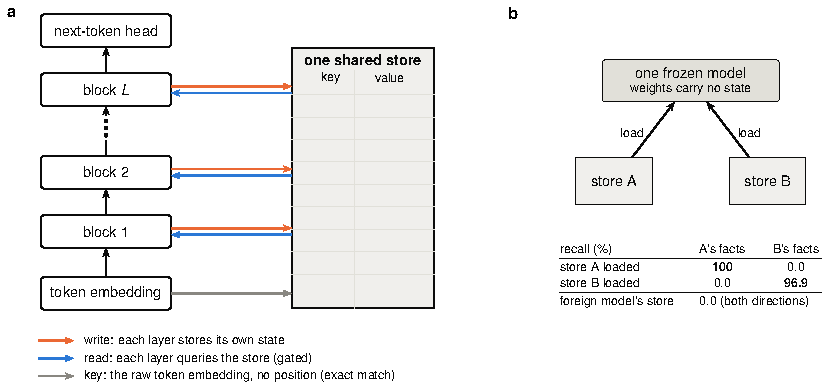
\includegraphics{fig1_architecture.pdf}
\caption{\textbf{Memory as a block.} \textbf{a}, Every layer reads from and writes its own
state into one shared store (orange arrows, writes; blue arrows, reads; grey arrow, the key). A
slot's key is the raw layer-0 token embedding without position, so retrieval is an exact token
match. Reads enter the residual stream through a gate that starts at zero, and the model keeps
no key--value cache between 128-token segments. \textbf{b}, The weights are stateless and the
store is the state. With the model frozen, loading the store that holds the queried facts gives
full recall and loading the other gives none. A store written by a differently seeded model
reads at 0\% although its facts are present, because its keys are the writer's embeddings.
$n=32$ queries per cell; 95\% intervals are in Table~1.}
\label{fig:arch}
\end{figure}

\begin{table}[p]
\centering
\small
\caption{\textbf{Core recall results.} Facts are stated once and queried out of context.
Recall is the exact match of the answer token on $n$ independent queries, with 95\% Wilson
score intervals (Methods). No hypothesis tests were used. Rows with two seeds list each
seed, and controls run at matched settings. Source data: Source Data Table~1.}
\label{tab:core}
\setlength{\tabcolsep}{4pt}
\begin{tabular}{@{}llrrl@{}}
\toprule
Experiment & Condition & $n$ & Recall (\%) & 95\% interval \\
\midrule
Facts in PG-19 prose,        & 8 facts  & 640 & 100.0 & 99.4--100.0 \\
single-token keys            & 16 facts & 640 & 100.0 & 99.4--100.0 \\
                             & 32 facts & 640 & 100.0 & 99.4--100.0 \\
                             & 64 facts & 640 & 99.1 & 98.0--99.6 \\
                             & scrambled store (64 facts) & 640 & 0.16 & 0.0--0.9 \\
\midrule
Persistence                  & store reloaded in a fresh process & 160 & 100.0 & 97.7--100.0 \\
                             & mismatched store file & 160 & 0.0 & 0.0--2.3 \\
\midrule
Placement (cold start,       & mean of all layers in one slot per token & 640 & 80.8 & 77.5--83.6 \\
32 facts)                    & each layer writes its own slot, seed 0 & 640 & 95.5 & 93.6--96.8 \\
                             & each layer writes its own slot, seed 1 & 640 & 98.9 & 97.8--99.5 \\
                             & same slots keyed by residual (control) & 640 & 0.2 & 0.0--0.9 \\
\midrule
Store as state               & store A loaded, A's facts & 32 & 100.0 & 89.3--100.0 \\
(one frozen model)           & store B loaded, B's facts & 32 & 96.9 & 84.3--99.4 \\
                             & the other store loaded (either direction) & 32 & 0.0 & 0.0--10.7 \\
                             & scrambled store & 32 & 3.1 & 0.6--15.7 \\
\midrule
Store as state               & model 1, its own store & 640 & 98.8 & 97.6--99.4 \\
(two seeded models)          & model 2, its own store & 640 & 100.0 & 99.4--100.0 \\
                             & the other model's store (either direction) & 32 & 0.0 & 0.0--10.7 \\
\bottomrule
\end{tabular}
\end{table}

\begin{figure}[p]
\centering
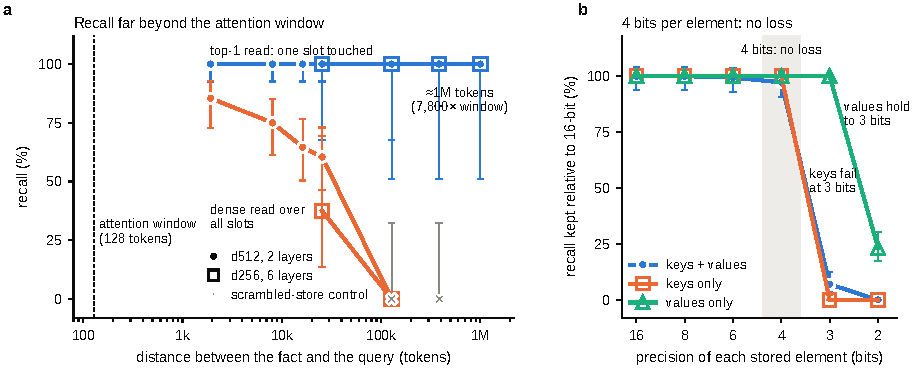
\includegraphics{fig2_longcontext.pdf}
\caption{\textbf{Recall far beyond the attention window, from a 4-bit store.}
\textbf{a}, Recall against the number of tokens between a fact and its query, for a two-layer
model (filled circles) and a six-layer model (open squares). A top-1 read, which uses one slot
(blue), stays at 100\% from 1.9k to 998k tokens, about 7,800 times the 128-token attention
window (dashed vertical line), whereas a dense read over all slots (orange) decays to 0\% by
128k tokens. Grey crosses, scrambled-store control. \textbf{b}, Recall when the stored codes are
quantized, relative to each model's unquantized recall, for keys and values together (blue
circles), keys only (orange squares) and values only (green triangles). Quantizing to 4 bits
(shaded) loses nothing and makes the store eight times smaller than at 32 bits. Keys fail at
3 bits; values hold to 3. The keys-and-values series uses a 64-fact model and the other two a
16-fact model. Error bars are 95\% Wilson intervals. In \textbf{a}, $n=48$ queries per point up
to 25k tokens and $n=4$--8 beyond (control, $n=8$), so the intervals at long range are wide; in \textbf{b}, $n=160$ per point, with the interval for the quantized recall divided by
the 16-bit recall. No hypothesis tests were used.}
\label{fig:long}
\end{figure}

\begin{figure}[p]
\centering
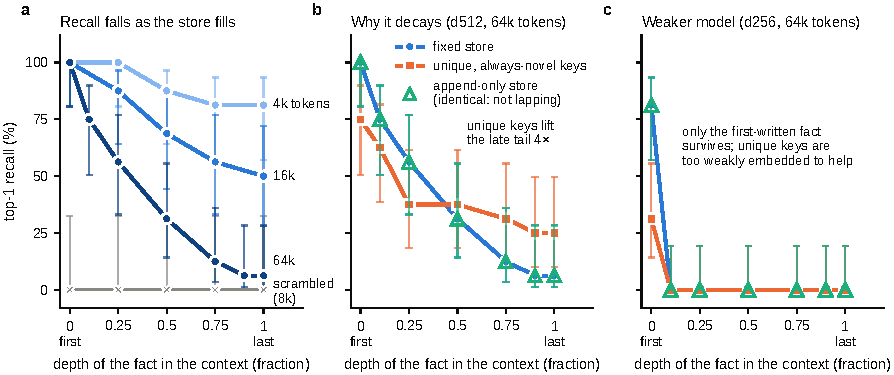
\includegraphics{fig3_passkey.pdf}
\caption{\textbf{No lost-in-the-middle, but a write-order limit.} Top-1 recall against the
depth at which the fact is written (0, first context window; 1, last before the query).
\textbf{a}, A two-layer model with 4k, 16k and 64k tokens of context (light to dark blue).
Recall falls monotonically with depth, so there is no mid-context dip, and late-written facts
are lost as the store fills. Grey crosses, scrambled store. \textbf{b}, Mechanism at 64k
tokens for the same model. An append-only store (green triangles) never overwrites and traces
a curve identical to the fixed store (blue circles). Keying facts on unique tokens, which always
pass the novelty gate (orange squares), lifts the late tail fourfold. \textbf{c}, The same for a
weaker six-layer model: only the first-written fact survives and unique keys do not help.
Panels \textbf{b} and \textbf{c} share the key. Error bars are 95\% Wilson intervals; $n=16$
queries per point (control, $n=8$). No hypothesis tests were used.}
\label{fig:passkey}
\end{figure}

\begin{figure}[p]
\centering
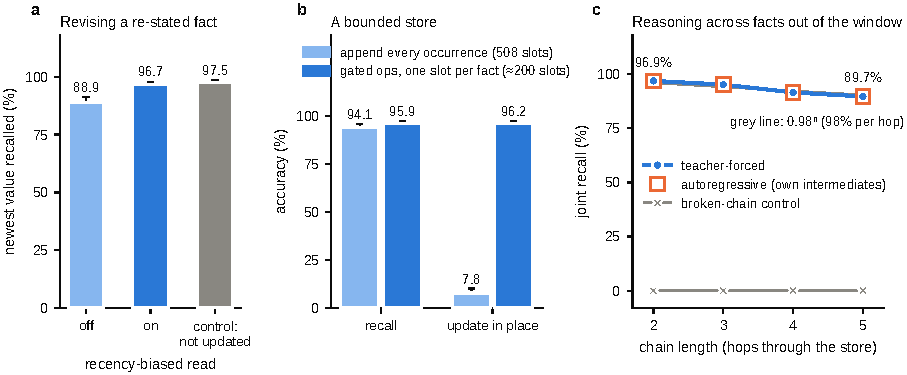
\includegraphics{fig4_memory.pdf}
\caption{\textbf{From a lookup table to a memory.} \textbf{a}, Revising a restated fact:
newest-value recall without (light blue) and with (dark blue) a recency-biased read, and for
facts that were never updated (grey). \textbf{b}, Gated write operations keep one slot per
fact: recall is maintained with about 200 slots (dark blue) instead of 508 (light blue), and
updates land in place. \textbf{c}, Multi-hop reasoning over facts held outside the context
window, by emitting each intermediate as a token and querying the store again: teacher-forced
(blue circles), autoregressive with the model's own intermediates (open orange squares) and with
one link of the chain broken (grey crosses). The grey line is 0.98 raised to the number of
hops. Two and three hops use 64 facts, four and five use 32. Error bars are 95\% Wilson
intervals; $n=640$ queries per bar or point. No hypothesis tests were used.}
\label{fig:memory}
\end{figure}


\end{document}
